\documentclass{article}

\usepackage{graphicx}
\usepackage{tikz}
\usepackage{tikzsymbols}
\usetikzlibrary{calc,patterns,shapes.geometric}
\pagestyle{empty}
\usepackage[margin=0pt]{geometry}
\geometry{papersize={14in,12in}}

\def\centerarc[#1](#2)(#3:#4:#5){\draw[#1] ($(#2)+({#5*cos(#3)},{#5*sin(#3)})$) arc (#3:#4:#5);}

\begin{document}
	\begin{figure}
		\centering
		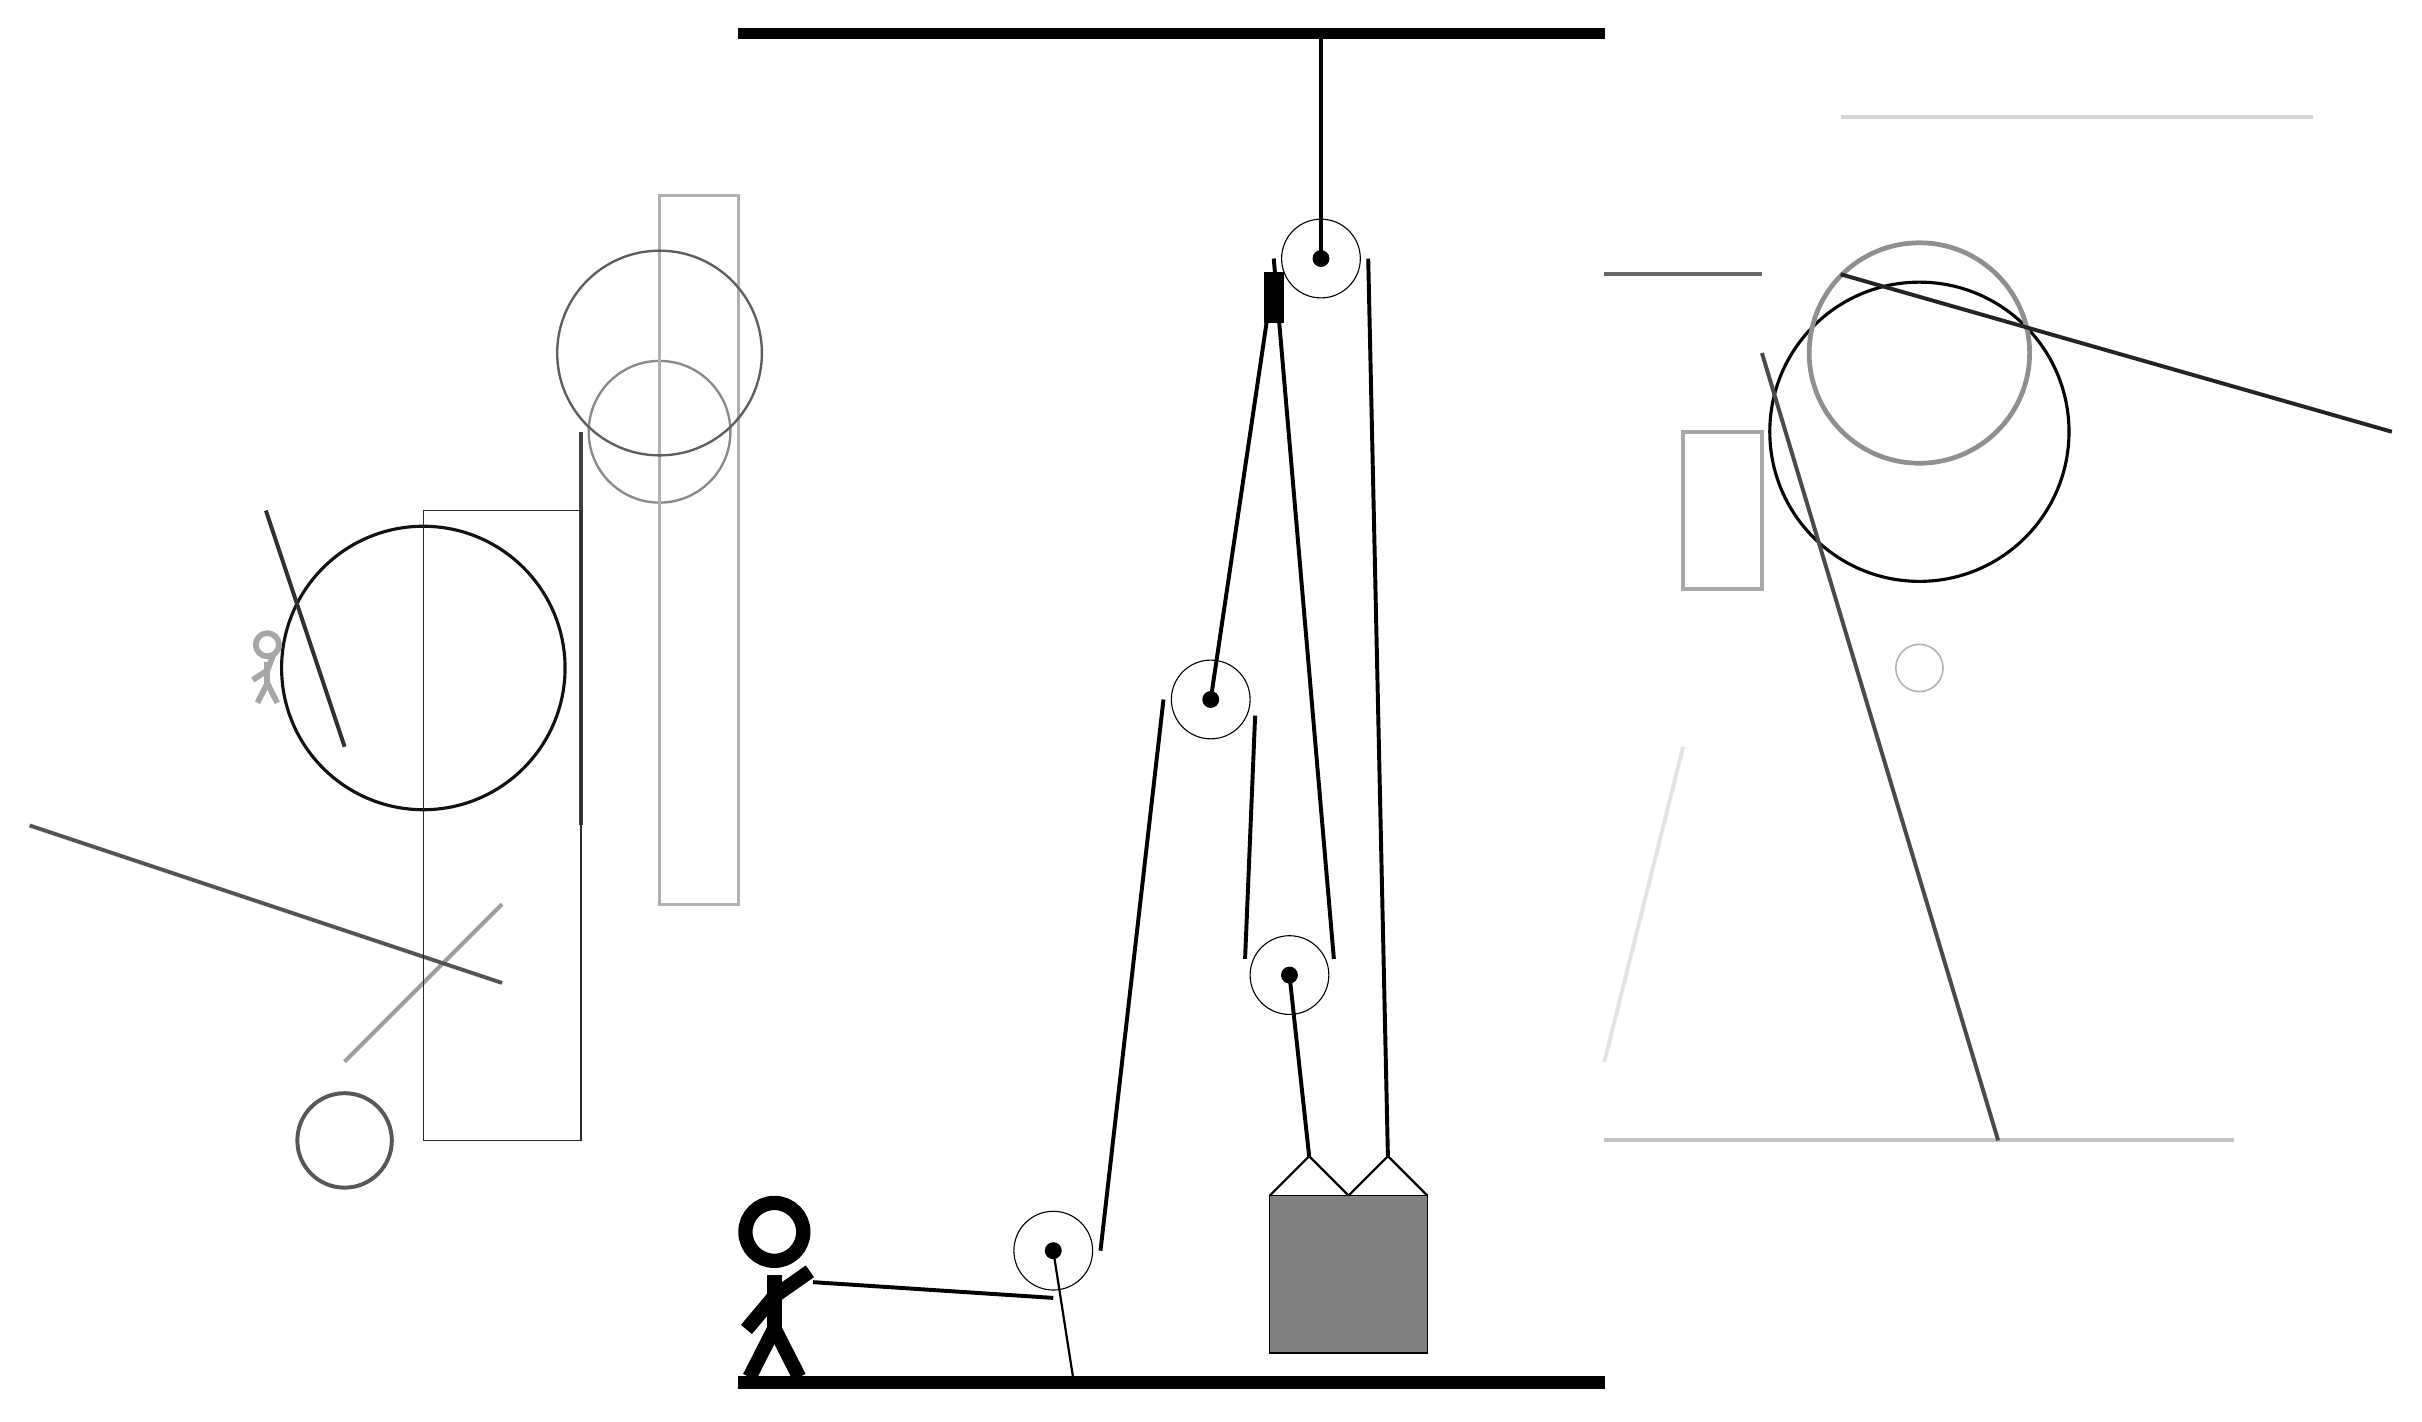
\begin{tikzpicture}
			%%%%% START %%%%%
			
			\draw[fill=black] (-6, 14) rectangle (5, 14.125);
			
			\draw (0, 5.6) circle (0.5);
			\draw[fill=black] (0, 5.6) circle (0.1);
			
			\draw (1, 2.1) circle (0.5);
			\draw[fill=black] (1, 2.1) circle (0.1);
			
			\draw (1.4, 11.2) circle (0.5);
			\draw[fill=black] (1.4, 11.2) circle (0.1);
			\draw[very thick] (1.4, 11.2) -- (1.4, 14);
			
			\draw (-2, -1.4) circle (0.5);
			\draw[fill=black] (-2, -1.4) circle (0.1);
			\draw[thick] (-2, -1.4) -- (-1.75, -3);
			
			\draw[line width=0.5mm, color=black!75](-8, 4) -- (-8, 9);
			
			\draw[line width=0.5mm, color=black!34] (7, 9) rectangle (6, 7);
			\draw[line width=0.5mm, color=black!23](5, 0) -- (13, 0);
			\draw[line width=0.5mm, color=black!17](8, 13) -- (14, 13);
			\draw[line width=0.5mm, color=black!38](-9, 3) -- (-11, 1);
			\draw [line width=0.3mm, color=black!46](-7, 9) circle (0.9);
			\draw[line width=0.4mm, color=black!31] (-6, 3) rectangle (-7, 12);
			
			\draw [line width=0.4mm, color=black!93](-10, 6) circle (1.8);
			\draw [line width=0.2mm, color=black!30](9, 6) circle (0.3);
			\draw[line width=0.5mm, color=black!67](-9, 2) -- (-15, 4);
			\node[line width=0.5mm, color=black!35] at (-12, 6) {\Strichmaxerl[4][33][69]};
			
			\draw [line width=0.4mm, color=black!98](9, 9) circle (1.9);
			\draw [line width=0.3mm, color=black!63](-7, 10) circle (1.3);
			\draw [line width=0.5mm, color=black!66](-11, 0) circle (0.6);
			\draw[line width=0.2mm, color=black!84] (-8, 0) rectangle (-10, 8);
			\draw[line width=0.5mm, color=black!59](5, 11) -- (7, 11);
			
			\draw [line width=0.6mm, color=black!44](9, 10) circle (1.4);
			
			\draw[line width=0.5mm, color=black!86](8, 11) -- (15, 9);
			\draw[line width=0.5mm, color=black!81](-11, 5) -- (-12, 8);
			
			\draw[line width=0.5mm, color=black!11](5, 1) -- (6, 5);
			\draw[line width=0.5mm, color=black!71](10, 0) -- (7, 10);
			
			
			
			\draw[thick]  (0.75, -0.7) -- (1.25, -0.2) -- (1.75, -0.7) -- (2.25, -0.2) -- (2.75, -0.7);
			\draw[fill=black!50] (0.75, -0.7) rectangle (2.75, -2.7);
			\draw[line width=0.5mm] (-5.05, -1.8) -- (-2, -2.0);
			\centerarc[line width=0.5mm](-2, -1.4)(270:360:0.6);
			\draw[line width=0.5mm] (-1.4, -1.4) -- (-0.6, 5.6);
			\draw[line width=0.5mm] (0, 5.6) -- (0.8, 11.0);
			\draw[line width=0.5mm, fill=black](0.7, 10.4) rectangle (0.9, 11.0);
			\centerarc[line width=0.5mm](0, 5.6)(-20:180:0.6);
			\draw[line width=0.5mm] (0.5638, 5.3948) -- (0.4362, 2.3052);
			\centerarc[line width=0.5mm](1, 2.1)(160:380:0.6);
			\draw[line width=0.5mm] (1.5638, 2.3052) -- (0.8, 11.2);
			\draw[line width=0.5mm](1, 2.1) -- (1.25, -0.2);
			\centerarc[line width=0.5mm](1.4, 11.2)(0:180:0.6);
			\draw[line width=0.5mm] (2.0, 11.2) -- (2.25, -0.2);
			
			\node at (-5.5, -1.9) {\Strichmaxerl[10][50][35]};
			
			\draw[fill=black] (-6, -3) rectangle (5, -3.15);
			
			%%%%% END %%%%%
		\end{tikzpicture}
	\end{figure}	
\end{document}